\documentclass[11pt,a4paper]{article}
\usepackage[margin=22mm,headheight=14pt,footskip=12mm]{geometry}
\usepackage[T1]{fontenc}
\usepackage{lmodern,microtype,amsmath,booktabs,tabularx,array,tikz,enumitem,fancyhdr,url}
\usepackage[hidelinks]{hyperref}
\urlstyle{same}
\usetikzlibrary{arrows.meta,positioning,calc}
\setlength{\parindent}{0pt}
\setlength{\parskip}{5pt plus 1pt}
\setlist{nosep,leftmargin=1.5em,topsep=3pt,itemsep=3pt}
\usepackage[font=small,labelfont=bf]{caption}
\pagestyle{fancy}\fancyhf{}\renewcommand{\headrulewidth}{0pt}\fancyfoot[L]{\small OPEP research proposal \textbar\ Revision 0.2}
\fancyfoot[R]{\small\thepage}
\makeatletter
\renewcommand\section{\@startsection{section}{1}{\z@}{10pt plus 2pt minus 2pt}{4pt}{\normalfont\large\bfseries}}
\renewcommand\subsection{\@startsection{subsection}{2}{\z@}{7pt plus 2pt}{3pt}{\normalfont\normalsize\bfseries}}
\makeatother
\hypersetup{pdftitle={Development of a Modular Experimental Platform for Multidisciplinary Engineering Research},pdfauthor={Abhijith Sivaprasadan},pdfsubject={Research proposal for technical discussion}}
\begin{document}
\begin{center}
{\LARGE\bfseries Development of a Modular Experimental Platform for Multidisciplinary Engineering Research\par}
\vspace{8pt}
{\large Abhijith Sivaprasadan\par}
Independent engineering research, Open Energy Methods\\
19 November 2026 \quad | \quad Working proposal for technical discussion
\end{center}
\vspace{3pt}
\noindent\textbf{Abstract.} This proposal concerns the development of a compact, reconfigurable test platform for mechanical, electrical, thermal-fluid and dynamic systems. The apparatus would share mechanical interfaces and measurement infrastructure across a number of small-scale experiments, with the aim of quantifying physical behaviour and testing numerical predictions against independent measurements. The initial work would address dimensional and assembly repeatability, structural compliance and electrothermal response, with further investigations considered according to available resources. Particular attention will be given to measurement uncertainty, the effect of boundary conditions and reproducibility. The designs, methods, software and resulting datasets are intended for free public access where release is permitted. The scope is preliminary; no physical measurements or experimental validation are reported here.

\section{Introduction}
Engineering models depend on assumptions about material properties, boundary conditions and the measurement process. Even relatively simple models can depart from measured behaviour when joint compliance, heat losses, sensor response or assembly variation are neglected. A small experimental platform provides a means of examining such differences without requiring a dedicated installation for every investigation.

Reconfigurable laboratory equipment is not a new concept. Ho et al. describe a low-cost vibration kit that supports several experiments using common hardware \cite{ho}. Lewis et al. demonstrate how a modular open benchtop flume can be characterized and documented for reproducible research and education \cite{lewis}. These examples motivate the use of replaceable test articles and openly documented construction. They do not establish novelty for the present proposal. A focused literature review will be undertaken for each investigation before any claim of original research is made.

\section{Research objectives}
The central question is whether a resource-constrained, reconfigurable platform can support reproducible measurements and quantitatively credible validation of models in several physical domains. The principal objectives are to:
\begin{enumerate}
\item Design and characterize common mechanical and instrumentation interfaces, including the effect of assembly and reassembly on measured quantities.
\item Investigate selected physical systems using analytical models, numerical simulations and controlled experiments, with explicit uncertainty and stated domains of validity.
\item Document the design, experimental procedures and analysis in sufficient detail for independent reproduction, criticism and adaptation.
\end{enumerate}
The work is an independent initiative (Open Physical Engineering Programme, OPEP). Access to the KTH EECS Student Workshop provides a possible practical route, not institutional sponsorship or approval of the proposed tests.

\newpage
\section{Proposed experimental platform}
The preferred initial concept is a baseplate carrying interchangeable fixtures and test articles, with removable instrumentation and a common data-acquisition procedure. It is intended to be dismantled and stored in one box; borrowed laboratory instruments are excluded from this packing constraint. The internal planning baseline uses a candidate 400 $\times$ 300 $\times$ 200 mm storage envelope and a 300 $\times$ 220 $\times$ 8 mm aluminium plate. These dimensions are provisional and must be assessed against actual workholding, stiffness, mass, packing, cost and component geometry. A split plate or simple extrusion frame may be more appropriate if it offers a better compromise.

\begin{center}
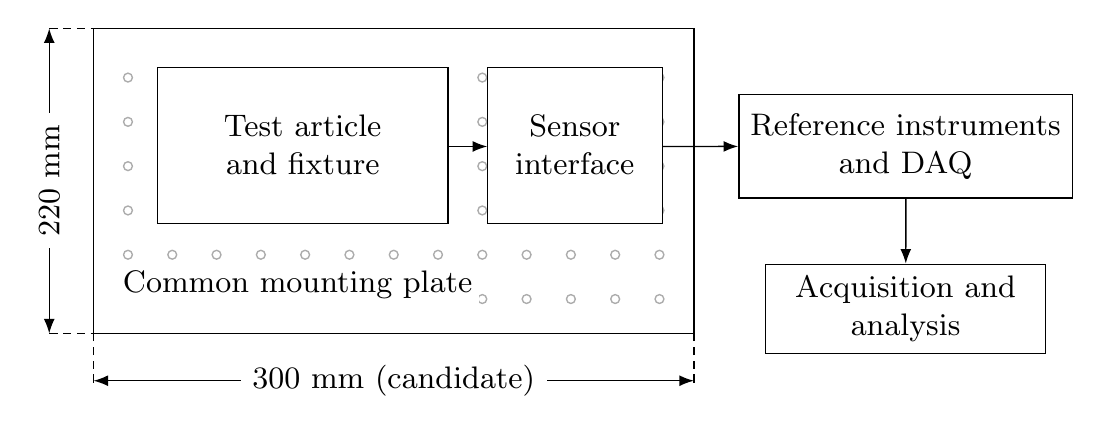
\begin{tikzpicture}[font=\small,>=Latex, line width=.5pt,scale=1.25,transform shape]
% top view
\draw (0,0) rectangle (6.1,3.1);
\foreach \x in {.35,.8,...,5.75}{\foreach \y in {.35,.8,...,2.75}{\draw[gray!65] (\x,\y) circle (.045);}}
\fill[white] (.65,1.12) rectangle (3.6,2.7); \draw (.65,1.12) rectangle (3.6,2.7);
\node[align=center] at (2.125,1.92) {Test article\\and fixture};
\fill[white] (4,1.12) rectangle (5.78,2.7); \draw (4,1.12) rectangle (5.78,2.7);
\node[align=center] at (4.89,1.92) {Sensor\\interface};
\draw[->] (3.6,1.9)--(4,1.9);
\node[draw,align=center,minimum width=2.85cm,minimum height=1.05cm] (daq) at (8.25,1.9) {Reference instruments\\and DAQ};
\draw[->] (5.78,1.9)--(daq.west);
\node[draw,align=center,minimum width=2.85cm,minimum height=.85cm] (pc) at (8.25,.25) {Acquisition and\\analysis};
\draw[->] (daq)--(pc);
\node[anchor=west,fill=white,inner sep=2pt] at (.22,.5) {Common mounting plate};
\draw[<->] (0,-.48)--(6.1,-.48) node[midway,fill=white] {300 mm (candidate)};
\draw[<->] (-.45,0)--(-.45,3.1) node[midway,rotate=90,fill=white] {220 mm};
\draw[densely dashed] (0,-.5)--(0,0) (6.1,-.5)--(6.1,0) (-.45,0)--(0,0) (-.45,3.1)--(0,3.1);
\end{tikzpicture}
\captionof{figure}{Conceptual arrangement of a replaceable test article and shared measurement chain (DAQ: data acquisition). Mounting pattern and dimensions are illustrative; this is not a manufacturing or wiring drawing.}
\end{center}

\subsection{Mechanical and electrical interfaces}
A common datum system and replaceable adapters would be used to define mount positions. Mounting force, fastener arrangement, orientation and contact surfaces would be recorded for each configuration. Reuse of a fixture does not imply that its thermal or mechanical boundary conditions remain unchanged. Any significant heat path or structural compliance introduced by the adapter should be characterized.

Electrical and sensor connections would be separated and selected for the specific circuit, including appropriate protection, isolation, grounding and strain relief. The instrument chain would be selected for each measurand rather than assuming that one acquisition device is suitable for both slow thermal transients and vibration measurements. Local protective measures and stop functions must not depend solely on software.

\subsection{Initial development}
The first stage would consist of a facility inventory, material selection, preliminary drawings, an assessment of dimensional accuracy and a simple unpowered mounting or structural experiment. A more elaborate PCB, CNC-machined fixture or dedicated controller would be developed only where necessary. The existing Electronics Bench Testing (EBT) work \cite{ebt} provides a preliminary electrothermal design and synthetic feasibility models; it remains a separate specialist workstream with its own qualification requirements. No existing numerical result is treated as experimental evidence.

For example, a cantilever test could compare measured tip displacement with the elastic prediction $\delta=FL^3/(3EI)$ under a known end load, then examine whether independently characterized mounting compliance improves the prediction. In the thermal study, heater terminal electrical power and surface temperatures would be measured separately; lead losses and heat bypass must be considered before interpreting an apparent thermal resistance as a physical convection parameter. Both studies require qualified instruments and a reviewed experimental configuration.

\newpage
\section{Candidate investigations}
The fifteen areas in the internal plan are grouped below into related investigations. Each retained study would have a narrower research question, specified response quantities and an appropriate reference or model. The order and extent of implementation are not fixed.

\begingroup\small\setlength{\tabcolsep}{5pt}\renewcommand{\arraystretch}{1.25}
\begin{tabularx}{\textwidth}{@{}>{\raggedright\arraybackslash}p{.22\textwidth}>{\raggedright\arraybackslash}X>{\raggedright\arraybackslash}p{.285\textwidth}@{}}
\toprule
Area & Proposed investigation and measured quantities & Principal resource or validation requirement\\
\midrule
Precision, manufacturing and production & Dimensional variation of machined or printed coupons; repeatability of locating interfaces after independent assembly. & Dimensional references, sufficient independent parts and remounts; tolerance and repeatability analysis.\\
Structural mechanics & Elastic force--deflection response of a beam or joint; effect of mounting compliance on prediction errors. & Known load, displacement measurement and geometry; analytical beam theory and finite element analysis (FEA).\\
Electronics and metrology & Accuracy and dynamic response of a low-energy sensing circuit or instrumentation board. & Reference electrical quantities, suitable meters and timebase; calibration and bandwidth checks.\\
Electrothermal engineering & Heater case and sink temperature histories under different mounting and cooling conditions; transferability of model parameters. & Qualified temperature channels, synchronized electrical power, safe operating envelope; EBT reduced-order models.\\
Thermal-fluid systems and turbomachinery & Pressure loss along interchangeable air ducts and guarded fan pressure--flow characteristics; effect on convective cooling. & Suitable differential pressure and flow references, fan speed and electrical input; correlations and computational fluid dynamics (CFD).\\
Control engineering & Identification of a bounded thermal or fan-speed plant; comparison of transient response under feedback control. & Qualified sensors and actuator, protected controller; held-out step responses and stability assessment.\\
Vibration and acoustics & Resonant frequencies, damping and frequency response; relation between structural vibration and acoustic spectra. & Suitable excitation, accelerometers and dynamic DAQ; calibrated microphone and controlled acoustic conditions for quantitative sound levels.\\
Environmental testing and reliability & Reversible effects of approved environmental exposures on drift and assembly behaviour. & Controlled exposure facility and qualified references; repeated baseline measurements.\\
Numerical modelling and condition monitoring & Analytical, reduced-order and higher-fidelity models; residual-based detection of bounded, non-destructive changes in operating conditions. & Verified model numerics, independently acquired validation data and sufficiently varied normal/fault conditions.\\
\bottomrule
\end{tabularx}
\captionof{table}{Preliminary investigations and evidence needed for their implementation. No row constitutes a commitment to conduct the experiment.}
\endgroup

The initial priority is to characterize the common interfaces and establish a defensible measurement chain. Structural and electrothermal work would follow if suitable instruments and permissions can be obtained. Later modules may use the same physical platform and data conventions, but their measurement requirements must be reviewed separately.

\newpage
\section{Research methodology}
\subsection{Experimental design and measurement}
Each experiment will begin with a defined measurand, boundary conditions, hypothesis or engineering question, and a preliminary estimate of the expected response. Pilot measurements will be used to establish suitable ranges, signal-to-noise ratios, stability and achievable precision before fixing the main test matrix. The design will use independent specimens or assembly events as the experimental units where appropriate. Sampling a single transient repeatedly does not constitute independent replication. Test order should be randomized or blocked where feasible, while documenting restrictions caused by warm-up, remounting or safety \cite{nist}.

The measurement chain will be documented with instrument identity, range, reference or calibration evidence, sampling interval, synchronization, sensor position and relevant environmental conditions. Uncertainty will be evaluated following the principles of the GUM \cite{gum}. For a differentiable measurement model $y=f(x_1,\ldots,x_n)$, the first-order combined standard uncertainty is
\begin{equation}
 u_c^2(y)=\sum_{i=1}^n\sum_{j=1}^n
 \frac{\partial f}{\partial x_i}\frac{\partial f}{\partial x_j}\,\mathrm{cov}(x_i,x_j).
\end{equation}
Instrument specifications, repeatability, calibration, sensor attachment, drift and correlated inputs will be considered as applicable. If measurement uncertainty is too large relative to the effect of interest, the experiment must be redesigned or its conclusions restricted.

\subsection{Numerical verification and experimental validation}
Models will first be checked against analytical solutions, limiting cases, conservation balances and numerical refinement where relevant. Calibration and validation data will be separated by independent test configuration or assembly where feasible; validation measurements will not be used retrospectively to tune the reported predictive model. Model discrepancies will be examined alongside experimental uncertainty and numerical error, following relevant verification and validation principles \cite{asme10,asme20}. Agreement will be reported only for the investigated quantities and conditions. The proposal does not claim formal conformity to these standards.

\section{Practical constraints and feasibility}
The KTH EECS Student Workshop lists metalworking, PCB milling, additive manufacturing, soldering, bench power supplies, oscilloscopes, signal generators and multimeters \cite{kthwork,kthmech,kthbio}. The presence of these equipment classes does not establish individual access, calibration, availability or suitability for a given experiment. In particular, suitable thermometry, synchronized DAQ, force and displacement references, flow and pressure instrumentation, accelerometers, calibrated microphones and environmental facilities have not been confirmed for this work.

This is a personal engineering hobby project undertaken in the author's spare time, without a fixed schedule or completion deadline. The scope is subject to equipment, instrumentation, materials, funding, expertise, time and continued workshop access. Each investigation will be assessed for scientific relevance, achievable uncertainty, cost, safety and reproducibility before procurement or fabrication. An investigation may be retained, simplified with a defensible change of method, deferred, or excluded entirely if its essential resources cannot realistically be secured. Reasons and changes to the scope will be recorded rather than substituting inadequate measurements for the required evidence.

All workshop work is subject to local rules and specific permissions. KTH requires supervision for machining activities and prohibits working alone or on live circuits \cite{kthmech,kthsafe}. Powered experiments require explicit confirmation of an allowed arrangement; otherwise, a separately authorized facility is needed or the work is omitted. High-voltage, pressure-vessel, combustion, destructive and exposed high-speed rotating experiments are outside the present scope.

\newpage
\section{Open research and request for technical feedback}
The intention is to make the engineering work freely accessible, including the original CAD and PCB files, drawings, bills of materials, calculations, experimental procedures, analysis code, raw measurements with metadata, uncertainty estimates and technical reports. Outputs will be released with appropriate open licences where ownership, third-party licensing, safety and facility requirements permit. Restrictions will be stated explicitly. The private workshop manuals are not part of the proposed public release. Data will be archived with configuration and revision identifiers; deviations, unsuccessful tests and negative results will be retained alongside successful measurements.

The present document is circulated before detailed design in order to obtain technical feedback from engineers, researchers and academics. Suggestions are particularly welcome on the following points:
\begin{itemize}
\item Relevant experimental investigations or industrial testing practices that could be implemented at small scale without compromising the validity of the measurements.
\item Potential weaknesses in the shared platform, mounting interfaces, experimental design, measurement methods or model-validation approach.
\item Comparable published experimental platforms, appropriate reference methods and practical ways to obtain essential instrumentation within reasonable constraints.
\end{itemize}
Suggestions will be reviewed against the engineering and scientific objectives, practical feasibility and relevant literature. Changes and the reasons for accepting, modifying or excluding proposed investigations will be documented in subsequent revisions. Contributions may be acknowledged with permission; substantive research contributions will be considered under appropriate authorship criteria.

The immediate next step is to establish the actual instrument inventory and workshop permissions before committing to a particular hardware configuration. This proposal is a working document, not an approved laboratory procedure or a report of completed experiments. Feedback is welcome through LinkedIn or the repository issue tracker: \url{https://github.com/Open-Energy-Methods/OPEP/issues}.

\begingroup\small\setlength{\parskip}{1pt}
\begin{thebibliography}{99}\setlength{\itemsep}{2pt}\setlength{\parsep}{0pt}
\bibitem{ho} I. Ho, A. H. Kumar and D. M. Harris, ``Reconfigurable mechanical vibrations laboratory kit,'' \emph{Journal of Open Hardware}, vol. 6, no. 1, article 4, 2022. \href{https://doi.org/10.5334/joh.40}{doi:10.5334/joh.40}.
\bibitem{lewis} M. Lewis, E. Silver, R. Hunt and D. M. Harris, ``OpenFlume: An accessible and reproducible benchtop flume for research and education,'' \emph{HardwareX}, vol. 20, e00583, 2024. \href{https://doi.org/10.1016/j.ohx.2024.e00583}{doi:10.1016/j.ohx.2024.e00583}.
\bibitem{ebt} Open Energy Methods, \emph{Electronics Bench Testing}, existing independent design and synthetic feasibility repository. \href{https://github.com/Open-Energy-Methods/electronics-bench-testing}{GitHub repository}.
\bibitem{nist} NIST/SEMATECH, \emph{e-Handbook of Statistical Methods}, Sec. 5.3, Choosing an experimental design. \href{https://www.itl.nist.gov/div898/handbook/pri/section3/pri3.htm}{Online handbook}.
\bibitem{gum} JCGM 100:2008, \emph{Evaluation of measurement data---Guide to the expression of uncertainty in measurement}. \href{https://doi.org/10.59161/JCGM100-2008E}{doi:10.59161/JCGM100-2008E}.
\bibitem{asme10} ASME V\&V 10, \emph{Standard for Verification and Validation in Computational Solid Mechanics}, 2019. \href{https://www.asme.org/codes-standards/find-codes-standards/standard-for-verification-and-validation-in-computational-solid-mechanics/2019}{ASME standard listing}.
\bibitem{asme20} ASME V\&V 20, \emph{Standard for Verification and Validation in Computational Fluid Dynamics and Heat Transfer}. \href{https://www.asme.org/codes-standards/find-codes-standards/standard-for-verification-and-validation-in-computational-fluid-dynamics-and-heat-transfer}{ASME standard listing}.
\bibitem{kthwork} KTH, \emph{Explore KTH's makerspaces}. \href{https://www.kth.se/en/student/kontakt/campus/makerspaces/explore/explore-1.1455863}{Student Workshop listing}. Accessed 19 Nov. 2026.
\bibitem{kthmech} KTH, \emph{Student Workshop: Mechanical manufacturing}. \href{https://www.kth.se/emp/student-workshop/verkstan/mekanik-1.686913}{Equipment and supervision}. Accessed 19 Nov. 2026.
\bibitem{kthbio} KTH, \emph{Student Workshop: Electronics}. \href{https://www.kth.se/emp/student-workshop/verkstan/elektronik-1.686912}{Electronics equipment}. Accessed 19 Nov. 2026.
\bibitem{kthsafe} KTH, \emph{Student Workshop: Order and Safety Rules}. \href{https://www.kth.se/emp/student-workshop/regler-och-sakerhet}{Safety rules}. Accessed 19 Nov. 2026.
\end{thebibliography}\endgroup
\end{document}
